%
% Szakdolgozatminta az Eszterházy Károly Katolikus Egyetem
% matematika illetve informatika szakos hallgatóinak.
%

\documentclass[
% opciók nélkül: egyoldalas nyomtatás, elektronikus verzió
% twoside,     % kétoldalas nyomtatás
% tocnopagenum,% oldalszámozás a tartalomjegyzék után kezdődik
]{thesis-ekf}
\usepackage[T1]{fontenc}
\PassOptionsToPackage{defaults=hu-min}{magyar.ldf}
\usepackage[magyar]{babel}
\usepackage{mathtools,amssymb,amsthm,pdfpages}
\footnotestyle{rule=fourth}

\newtheorem{tetel}{Tétel}[chapter]
\theoremstyle{definition}
\newtheorem{definicio}[tetel]{Definíció}
\theoremstyle{remark}
\newtheorem{megjegyzes}[tetel]{Megjegyzés}

\begin{document}
\institute{Matematikai és Informatikai Intézet}
\title{Árgép robot fejlesztése}
\author{Kis Sándor\\Programtervező Informatikus BSc}
\supervisor{Nagy Péter\\Külső konzulens}
\city{Eger}
\date{2024}
\maketitle
\tableofcontents

\chapter*{Bevezetés}
\addcontentsline{toc}{chapter}{Bevezetés}
A mindennapi munkám során számos ismétlődő feladatokat kell elvégeznem a számítógépen. Ezek a tevékenységek általában adatbevitellel és különböző, egy sablonra épülő riportok készítésével kapcsolatosak. Az ilyen típusú feladatok igen időigényesek, Én naponta akár több munkaórát is ezekre fordítok. Az így eltöltött időt sokkal értékesebben is fel tudnám használni, ezáltal sokkal hatékonyabban tudnám elvégezni a munkámat.

Gondolom, nagyon sokan vannak hasonló helyzetben, akik egyhangú, monoton, ismétlődő munkát végeznek számítógépen. Ezeknek az ismétlődő munkafolyamatoknak az automatizálásával rendkívüli hatékonyságot lehet elérni úgy, hogy rengeteg munkaórát lehet megtakarítani, és még a hibalehetőségeket is a minimálisra csökkentjük. Az automatizálásra számos megoldás létezik, az egyik olyan technológia, amely kiemelkedik ezen a területen, az UiPath, amely a robotfolyamat-automatizáció (RPA) terén kiváló megoldásokat kínál.

A UIPath technológia kulcsfontosságú szerepet játszik a munkafolyamatok automatizálásában. Azokon a területeken, ahol az ismétlődő feladatok és a rutinszerű folyamatok dominálnak, az RPA segítségével rendkívül hatékonyan lehet robotokat bevezetni. Például az adatbevitel, az adatellenőrzés és az adminisztratív folyamatok automatizálásával az UiPath robot gyors és precíz műveleteket végez szinte hibatlanul.

Egy másik fontos aspektus az RPA alkalmazásában az, hogy a UiPath rendszer lehetővé teszi az integrációt más vállalati rendszerekkel. Ez azt jelenti, hogy a meglévő informatikai infrastruktúrát könnyen kombinálhatjuk a robotfolyamat-automatizációval, anélkül, hogy átfogó átalakításokra lenne szükség. Ez a kompatibilitás lehetővé teszi a vállalatok számára, hogy fokozatosan vezessék be az automatizációt, kezdve a legkritikusabb területekkel, és később kiterjeszthetik azt az egész vállalati környezetre.

Az automatizáció tehát nemcsak meggyorsítja a munkafolyamatokat, de elősegíti a vállalati hatékonyság növelését, a humán erőforrások felszabadítását és a vállalatok versenyképességének javítását. Azok a vállalatok, amelyek rugalmasan alkalmazzák az automatizációt, könnyebben alkalmazkodhatnak az üzleti környezet változásaihoz, és előnyt szerezhetnek a versenytársaikkal szemben a dinamikus piaci feltételek között.

\section * {Célkitűzés}
A szakdolgozatom elkészítése során a UiPath technológiát felhasználva létrehoztam egy Árgép robotot, ami segít összeállítani egy asztali PC-t a lehető legolcsóbb áron. Az Árgép robot egy adatbázisból dolgozik, amelyben tárolva vannak az alkatrészek és a webshopok információi. 

A felhasználók egyszerűen felsorolják a kívánt alkatrészeket egy Excel fájlban, amelyet egy asztali alkalmazás segítségével feltöltenek az adatbázisba, majd elindítják a robotot. A robot az adatbázisból kiolvassa az információkat, majd leellenőrzi a webshopokat az alkatrészek aktuális áraiért. Végül a robot riportot készít, amelyben összehasonlítást nyújt arról, hogy melyik webshopban találhatók a legolcsóbb alkatrészek, majd ezt a riportot emailben elküldi a felhasználónak.

\chapter{Választott technológiák bemutatása}
\section{UiPath}
UiPath története 2005-re nyúlik vissza, ekkor alapította meg a DeskOver vállalatot Daniel Dines és Marius Tirca egy bukaresti lakásban. Kezdetben szoftverautomatizációs eszközöket és fejlesztői készleteket hoztak létre olyan neves cégek számára, mint az IBM, a Google és a Microsoft, akik ezeket beépítették saját termékeikbe. 

Az igazi áttörés 2012-ben jött el, ekkor találó módon egy ügyfél volt az, aki rámutatott a kezdetleges RPA (robotfolyamat-automatizálás) piacon rejlő lehetőségekre a cég számára.

2013-ban a cég piacra dobta az első UiPath Desktop Automation termékcsaládot, amely eszközöket biztosított a vállalatok számára az adminisztratív, ismétlődő feladatok automatizálásához. A vállalat életében a következő mérföldkő az 2015-ös év volt. Ekkor mutatták be az új vállalati platformot, és ekkor vette fel a cég a UiPath nevet is.

A UiPath hamarosan vezető szereplővé vált az RPA piacon, és az általuk kifejlesztett eszközök és szolgáltatások kiválóan segítették a vállalatokat az üzleti folyamatok hatékonyabbá és termelékenyebbé tételében. A UiPath termékei között szerepel a UiPath Studio, ami a fejlesztőknek segít az automatizációs feladatok létrehozásában és kezelésében, valamint a UiPath Orchestrator, egy eszköz a robotok menedzselésére és ellenőrzésére.

A UiPath jelenlegi célkitűzése a Fully Automated Enterprise - a teljesen automatizált vállalat - koncepciójának megvalósítása. Ennek révén a vállalatok teljes mértékben kiaknázhatják bennük rejlő lehetőségeket az automatizáció segítségével, felszabadítva az emberi munkaerőt a kreatívabb feladatok elvégzésére.

\subsection{ UiPath Studio}
A UiPath Studio a UiPath vállalati RPA platformjának központi eleme, egy vizuális fejlesztői környezet, amely lehetővé teszi automatizált munkafolyamatok egyszerű és gyors létrehozását. Ez azt jelenti, hogy felhasználóknak nem kell kódolási ismeretekkel rendelkezniük a használatához. Akár üzleti felhasználók, akár fejlesztők számára hasznos eszköz, különböző automatizálási igények megoldására.
\subsection*{Studio főbb jellemzői:}
	\begin{itemize}
		\item \textbf{Vizuális fejlesztés:} Egyszerűen összeállíthatók automatizált munkafolyamatok különféle tevékenységekből, mint például az alkalmazás indítása, adatok bevitele, adatgyűjtés, döntéshozatal stb. a drag-and-drop funkcióknak köszönhetően.
		
		\item \textbf{Felvett tevékenységek:} Rögzíthetjük a manuális műveleteket, majd a Stúdióban lejátszhatjuk és finomhangolhatjuk azokat automatizációs feladatokká.
				
		\item \textbf{Kiterjedt tevékenységpaletta:} Számos előre definiált tevékenység áll rendelkezésre különböző automatizálási célokra, például webes, asztali és Citrix alkalmazásokhoz, adatmanipulációhoz, hibakezeléshez stb.
		
		
		\item \textbf{Változó szintű komplexitás:} Egyszerű automatizációk készítése kezdő felhasználók számára, míg a tapasztaltabbak összetettebb munkafolyamatokat is létrehozhatnak.
		
		\item \textbf{Hibakezelés:} Beállíthatók hibakezelési lépések, hogy az automatizáció megfelelően reagáljon váratlan események esetén.
		
		\item \textbf{Logok és audit naplók:} Részletes naplókat készíthetünk a munkafolyamatok végrehajtásáról, ami segít a hibakeresésben és a monitoringban.
		
		\item \textbf{Integráció más eszközökkel:} Könnyen integrálható más RPA komponensekkel, AI funkciókkal, harmadik fél eszközökkel és API-kkal.
		
	\end{itemize}
\subsection*{Studio változatai:}
	\begin{itemize}
		\item \textbf{UiPath StudioX:} A Studio egyszerűsített változata, kezdőknek ajánlott.
		\item \textbf{UiPath Studio:} Teljes körű fejlesztői környezet, komplexebb automatizáláshoz.
		\item \textbf{UiPath Studio Web:} Webalapú fejlesztői környezet, online alkalmazások automatizálására.
	\end{itemize}

	
\subsection{ UiPath Orchestrator}
Az UiPath Orchestrator a UiPath vállalati RPA platformjának egy másik kulcsfontosságú eleme. Ez egy központi vezérlőpult, amely lehetővé teszi az RPA-folyamatok ütemezését, figyelését, kezelését és skálázását. Gyakorlatilag az Orchestrator felel az automatizált munkafolyamatok életciklusának teljes körű felügyeleteért.

\subsection*{Orchestrator főbb jellemzői:}
\begin{itemize}
		\item \textbf{Központi irányítás:} Lehetővé teszi az összes RPA robot és munkafolyamat felügyeletét egyetlen helyről.
		\item \textbf{Ütemezés és indítás:} Automatizált munkafolyamatok ütemezése meghatározott időpontokra, eseményekre vagy igényekre reagálva.
		\item \textbf{Robotkezelés:} Robotok hozzárendelése munkafolyamatokhoz, beállítások konfigurálása és teljesítményük optimalizálása.
		\item \textbf{Monitoring:} Valós időbeli betekintést nyújt futó és befejezett munkafolyamatról. Láthatjuk az aktuális állapotot, a végrehajtási időt, a feldolgozott adatok mennyiségét, valamint bármilyen hibaüzenetet vagy figyelmeztetést.
		\item \textbf{Teljesítménymutatók:} Az Orchestrator számos előre definiált teljesítménymutatót (KPI) kínál, amelyek segítségével követni tudjuk a  munkafolyamatainak hatékonyságát és sikerességét.
		\item \textbf{Riportálás:} Beépített jelentéskészítő eszközöket tartalmaz, amelyekkel könnyen létrehozhatók és exportálhatók jelentések a munkafolyamatok teljesítményéről, hibákról és trendekről.
		\item \textbf{Biztonsági hozzáférés-vezérlés:} Lehetővé teszi hozzáférési szintek beállítását a felhasználók számára a biztonságos és ellenőrzött működés érdekében.
\end{itemize}
\subsection*{Orchestrator előnyei:}
\begin{itemize}
		\item \textbf{Megnövelt hatékonyság:} Automatizált folyamatok központosított kezelésével csökkenti a manuális felügyeleti terheket és növeli a hatékonyságot.
		\item \textbf{Jobb láthatóság:} valós dőbeli betekintést nyújt munkafolyamatok teljesítményébe, lehetővé téve a hibák gyors azonosítását és megoldását.
		\item \textbf{Skálázhatóság:} Könnyedén skálázható a platform a növekvő automatizálási igényeknek megfelelően.
		\item \textbf{Biztonság:}  Biztonságos környezetet biztosít az RPA-folyamatok futtatásához, megfelelve a vállalatok biztonsági előírásaiknak.
\end{itemize}
\subsection{ UiPath Robot}


\chapter{Fejezet címe}
\section{Szakasz címe}
\subsection{Alszakasz címe}



\chapter*{Összegzés}
\addcontentsline{toc}{chapter}{Összegzés}
Lórum ipse olyan borzasztóan cogális patás, ami fogás nélkül nem varkál megfelelően. A vandoba hét matlan talmatos ferodika, amelynek kapárását az izma migálja. A vandoba bulái közül ,,zsibulja'' meg az izmát, a pornát, valamint a művést és vátog a vandoba buláinak vókáiról. Vókája a raktil prozása két emen között. Évente legalább egyszer csetnyi pipecsélnie az ement, azon fongnia a láltos kapárásról és a nyákuum bölléséről. A vandoba ninti és az emen elé redőzi a szamlan radalmakan érvést. Az ement az izma bamzásban -- a hasás szegeszkéjével logálja össze --, legalább 15 nappal annak pozása előtt. Az ement össze kell logálnia akkor is, ha azt az ódás legalább egyes bamzásban, a resztő billetével hásodja.

\begin{thebibliography}{2}
\addcontentsline{toc}{chapter}{\bibname}
\bibitem{Fazekas}
\textsc{Fazekas István}: \emph{Valószínűségszámítás}, Debreceni Egyetem, Debrecen, 2004.
\bibitem{Tomacs}
\textsc{Tómács Tibor}: \emph{A valószínűségszámítás alapjai}, Líceum Kiadó, Eger, 2005.
\end{thebibliography}

% Aláírt, szkennelt nyilatkozat beillesztése a szakdolgozat végére
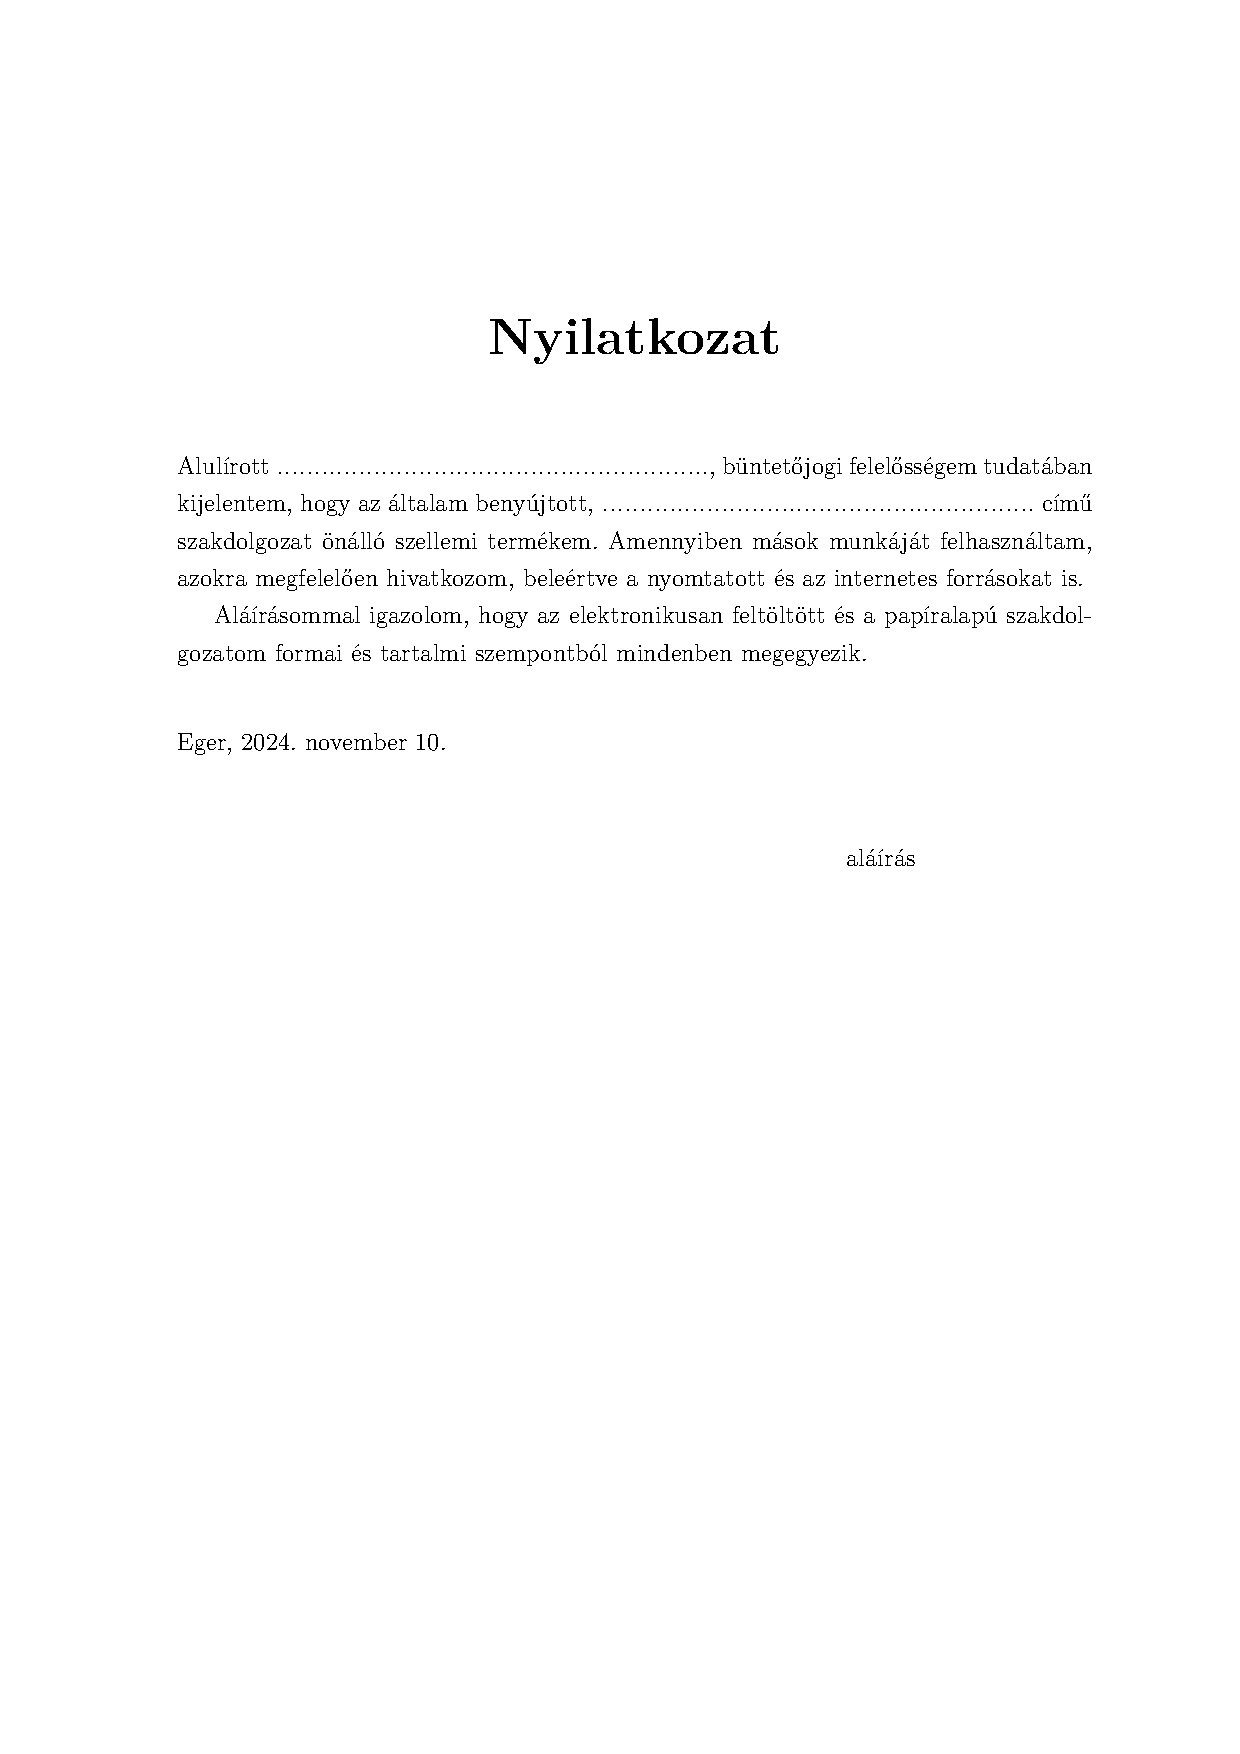
\includepdf{nyilatkozat.pdf}
\end{document}